\begin{figure}[h]
    \centering
    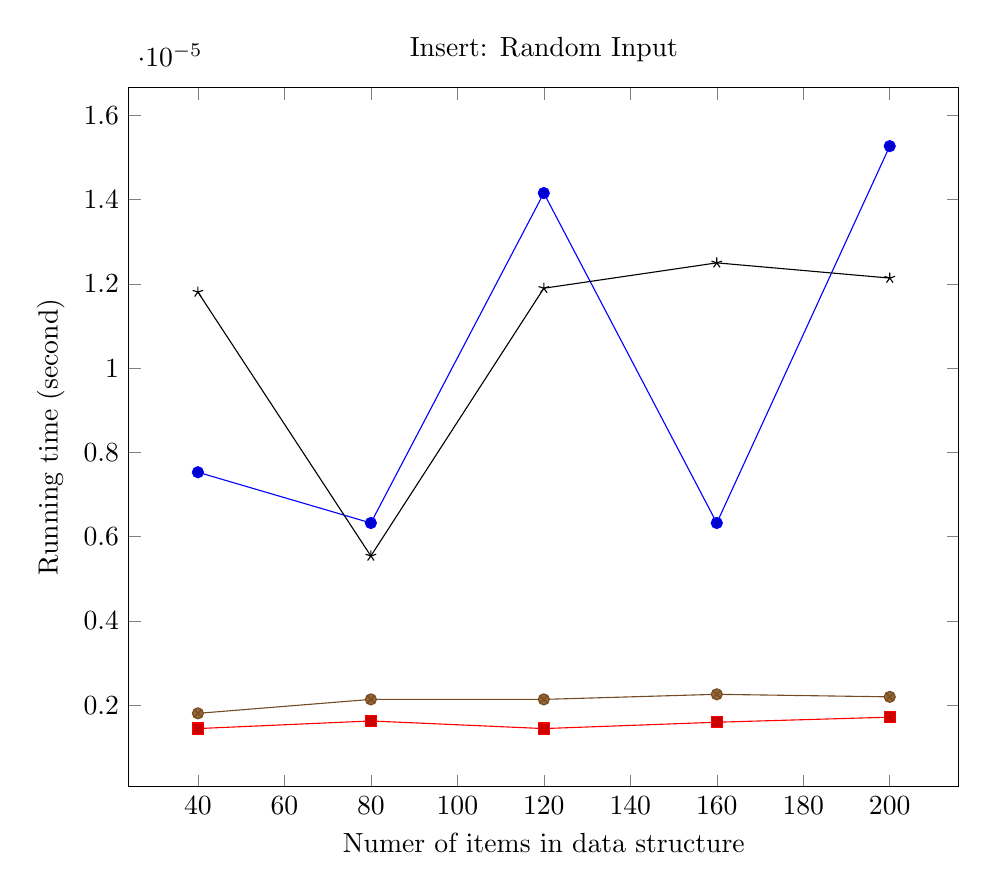
\begin{tikzpicture}
        \begin{axis}[
            xlabel={Numer of items in data structure},
            ylabel={Running time (second)},
            title={Insert: Random Input},
            width=\textwidth
        ]
		\addplot coordinates {
			(40, 7.529383418791724e-06)
			(80, 6.324682071784382e-06)
			(120, 1.4155240827323779e-05)
			(160, 6.324682071784382e-06)
			(200, 1.526958957331348e-05)
		};
		\addplot coordinates {
			(40, 1.4456416164043695e-06)
			(80, 1.6263468184563034e-06)
			(120, 1.4456416164043695e-06)
			(160, 1.5962292847837566e-06)
			(200, 1.716699419485046e-06)
		};
		\addplot coordinates {
			(40, 1.8070520205082374e-06)
			(80, 2.1383448909395585e-06)
			(120, 2.1383448909395585e-06)
			(160, 2.258815025635297e-06)
			(200, 2.198579958284652e-06)
		};
		\addplot coordinates {
			(40, 1.180607320066529e-05)
			(80, 5.541626196231553e-06)
			(120, 1.1896425801694033e-05)
			(160, 1.2498776475194929e-05)
			(200, 1.2137366071096612e-05)
		};
        \legend{}
        \end{axis}
    \end{tikzpicture}
    \caption{Average of 0 operations, benchmarked every 0, starting at 0.}
\end{figure}